\section{遺伝的アルゴリズム}
\subsection{概要}
本研究の目的は、ブラックジャックにおいてプレイヤーの利得を増加させ、かつ定義した
複雑性がより小さくなるような戦略を発見することである.そのために我々はプレイヤーの
勝率、戦略の複雑性の数値から性能1、性能2という2つの評価値を設定した。
戦略はプレイヤーの手札、ディーラーのアップカードを軸とする表で表される。評価値を
大きくするような戦略を見つけることは、一般的には最適化問題と分類される。
本研究で扱っているブラックジャックというゲームは、既に使用されたカードによって
後のプレイにおける、カードの出現確率が変動する。そのため単純な式でゲームの進行を表現するのは
現在のところ困難であり,プレイヤーの行動とゲームの結果のみを用いて戦略の最適化を
行う必要がある。

また、ブラックジャックの戦略は18行10列の表で表すことができる。単純にヒット、スタンドを行うという制限を
付けた場合でも、2の180乗通りの戦略表が考えられる。この通り数は膨大であり、単純に全探索を行うには非現実的な
時間を要する。

そのため本研究では入出力の関係から最適なパラメータを探索するアルゴリズムのなかで,生物の進化過程を模した、遺伝的アルゴリズム
という手法によって最適な戦略を発見することを試みた.遺伝的アルゴリズムは数ある探索対象の中から効率的に解を探索するため、
膨大な探索範囲を持つ戦略表に対して適していると考え使用した。
\bunseki{※米村祥裕}

\subsection{アルゴリズムの説明}
遺伝的アルゴリズムは生物の遺伝メカニズムをアイデアの中心として考案された最適化アルゴリズムの一つである。遺伝的アルゴリズムは次の工程からなる。
  \begin {enumerate}
    \item 初期個体群の生成
    \item 各個体の環境への適応度の評価
    \item 選択アルゴリズムによって次世代個体の親となる個体を抽出
    \item 交叉アルゴリズムによって親個体から次世代個体を生成
    \item 次世代個体に対して突然変異を適用
    \item 2から4を、次世代個体が必要数に達するまで繰り返し実行
    \item 2から5を、適応度が一定以上になるか最大世代になるまで繰り返し実行
  \end {enumerate}

本プロジェクトにおいて、個体とは戦略表に相当し、環境への適応度は、ブラックジャックをプレイした時の性能に相当する。

これから、遺伝的アルゴリズムにおいて個体がどのように表現されるのかについて遺伝子コーディングという項目で説明する。
また遺伝子コーディングの説明を使って、選択アルゴリズム、交叉アルゴリズム、突然変異について説明する。

\bunseki{※米村祥裕}

\subsection{遺伝子コーディング}
遺伝子コーディングとは探索対象となっている問題を遺伝子配列として扱うために対応させる作業である。生物の遺伝子には遺伝子型(genotype)と表現型(phenotype)とがある。
遺伝子型とは遺伝子の配列のことで、表現型とは遺伝子型によって現れる形質のことである。そのため遺伝子型として存在していても発現しない形質も当然存在する。遺伝子コーディングにおいては
探索対象においての一つの解パターンが表現型、解パターンを表現するための情報配列が遺伝子型に対応する。情報配列としては単純に0と1のいずれかの数値を要素としてもつバイナリ配列や
順序関係を番号で表した順序配列、または文字配列などがある。巡回セールスマン問題で遺伝的アルゴリズムを適用する場合には順序配列に巡回順序をそのまま記述するなど、情報配列がそのまま表現型になる場合もある。

本プロジェクトにおいて、遺伝的アルゴリズムを使用したシミュレーションでは、ヒットとスタンドからなる戦略についてのみ探索を行ったため、バイナリ配列を用い、表現型として現れる
戦略は、配列上の対応する位置の要素が0であればヒット、1であればスタンドであるという変換によって遺伝子コーディングを実装した。
\bunseki{※米村祥裕}

\subsection{選択アルゴリズム}
\subsubsection{ルーレット選択方式}
ルーレット選択方式とは、各個体が選ばれる確率を、適応度に比例する式で決定するアルゴリズムである。そのため適応度比例選択方式とも呼ばれる。
ルーレット選択方式において、各個体$i$の適応度を$f_i$として、個体$i$が親個体として選択される確率$P(i)$は次の式で定義される。
$$P(i) = \frac{f_i}{\sum_k f_k}$$
\subsubsection{エリート保存方式}
エリート保存方式とは現世代における、最大の適応度である個体を次世代個体に登録する方式である。ルーレット選択では、親個体の選択が確率的に行われることから、
次世代個体が現世代個体の性能を下回ることが十分に考えられる。そこで、最大の性能の個体を次世代でも作ることで性能の低下を防ぐことができる。
\bunseki{※米村祥裕}

\subsection{交叉アルゴリズム}
\subsubsection{一様交叉アルゴリズム}
一様交叉アルゴリズムでは、まず個体の遺伝子長と同じ大きさのバイナリ配列を生成する。この時バイナリ配列上には0と1が並ぶが、各要素が0と1のいずれに
なるかはランダムに決定する。こうしてできたバイナリ配列をビットマスクという。2つの親個体の対応する遺伝子を$K_1, K_2$として,それらの遺伝子に対応する
ビットマスク上の要素を$M$と表記する。$M$の値に応じて次のように交叉を適用し、次世代個体$k_1, k_2$を生成する。
  \begin{itemize}
    \item $M = 0$なら$k_1 \leftarrow K_2, k_2 \leftarrow \overline{K_1}$
    \item $M = 1$なら$k_1 \leftarrow K_1, k_2 \leftarrow K_1$
  \end{itemize}
遺伝子長と同じ長さのマスクを生成し、対応するマスクの値によって交叉を変化させるものであれば一様交叉と言われるため、上記のものとは異なる実装も考案されている。
\bunseki{※米村祥裕}

\subsection{突然変異アルゴリズム}
個体に変化が起きなくなると、新しい解を探索することができなくなるため、それを防ぐために個体の遺伝子情報をランダムに変化させるのが
突然変異アルゴリズムである。突然変異アルゴリズムでは、生成されたすべての次世代個体のすべての遺伝子配列上要素について、あらかじめ設定した
確率で次の変更を行う。
  \begin{itemize}
    \item 元の要素が0なら1にする
    \item 元の要素が1なら0にする
  \end{itemize}
\bunseki{※米村祥裕}

\subsection{実験条件}
遺伝的操作についてのパラメータは表に示すように設定した。

  \begin{table}[htb]
    \centering
    \label{geneticparameter}
    \caption{遺伝的操作のパラメータ}
    \begin{tabular}{|c|c|} \hline
      遺伝子長 & 180 \\ \hline
      個体数 & 200 \\ \hline
      適応度 & 勝率 $\div$ 複雑性 \\ \hline
      最大世代数 & 10000 \\ \hline
      交叉率 & 0.85 \\ \hline
      突然変異率 & 0.006 \\ \hline
    \end{tabular}
  \end{table}

個体数の設定については様々な方針が提案されているが、今回は遺伝子長よりも多い数の個体を用意するというものにした。
突然変異率については遺伝子長の逆数とするという方法が考案されていたため、採用した。今回の場合だと$1/180$となっている。

ブラックジャックのゲームを行うときの条件は次のように設定した。

\begin{itemize}
\item デック数は無限
\item ゲーム数は5万回
\end{itemize}

ベーシックストラテジーと比較するため、前提条件として無限デックである設定にしてゲームを行わせた。
\bunseki{※米村祥裕}

\subsection{実験結果}
遺伝的アルゴリズムによるシミュレーションを行った結果、図に示すような性能の推移となった。図中のmaxは最優秀性能の個体の適応度を
表している。minは最低性能の個体の適応度、meanは全個体の適応度の平均値、medianは全個体の適応度の中央値、top\_meanは上位10個体の適応度の平均値、
top\_medianは上位10個体の適応度の中央値を表している。

  \begin{figure}[htbp]
    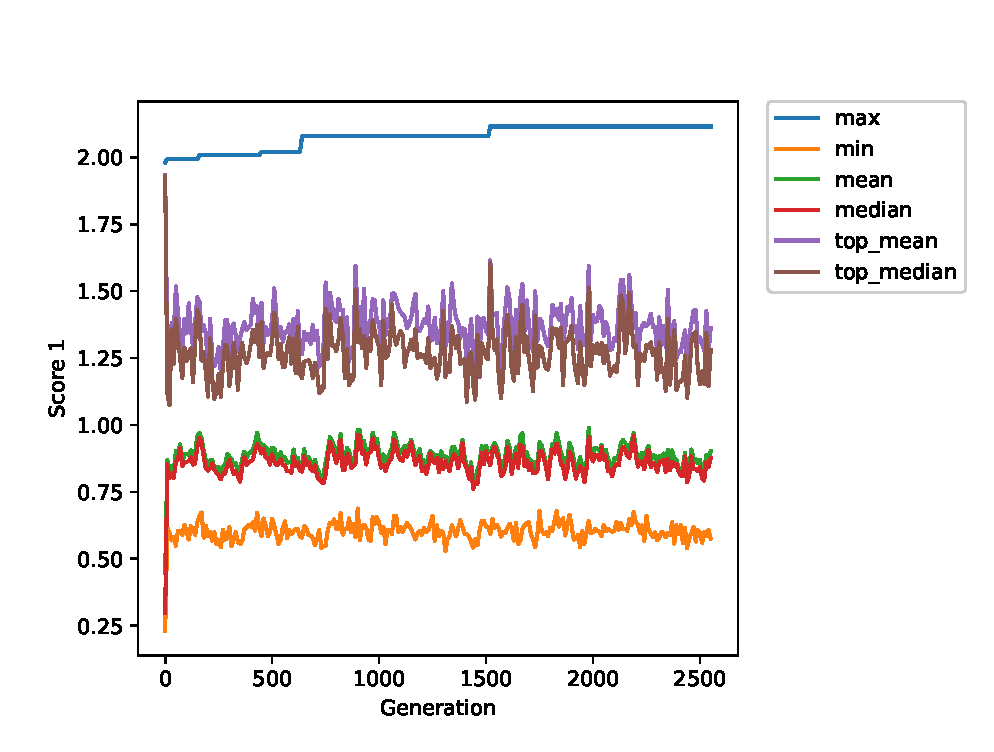
\includegraphics[width=14.0cm]{figure/gaprocess.eps}
    \caption{遺伝的アルゴリズムによるシミュレーションの進行}
    \label{gaprocess}
  \end{figure}

\bunseki{※米村祥裕}

\section{まとめ・手法の問題点}